\documentclass[paper=a4, fontsize=11pt]{scrartcl}
\usepackage[T1]{fontenc}
\usepackage{fourier}
\usepackage{listings}
\usepackage[english]{babel}															% English language/hyphenation
\usepackage[protrusion=true,expansion=true]{microtype}	
\usepackage{amsmath,amsfonts,amsthm} % Math packages
\usepackage[pdftex]{graphicx}	
\usepackage{url}


%%% Custom sectioning
\usepackage{sectsty}
\allsectionsfont{\centering \normalfont\scshape}


%%% Custom headers/footers (fancyhdr package)
\usepackage{fancyhdr}
\pagestyle{fancyplain}
\fancyhead{}											% No page header
\fancyfoot[L]{}											% Empty 
\fancyfoot[C]{}											% Empty
\fancyfoot[R]{\thepage}									% Pagenumbering
\renewcommand{\headrulewidth}{0pt}			% Remove header underlines
\renewcommand{\footrulewidth}{0pt}				% Remove footer underlines
\setlength{\headheight}{13.6pt}


%%% Equation and float numbering
\numberwithin{equation}{section}		% Equationnumbering: section.eq#
\numberwithin{figure}{section}			% Figurenumbering: section.fig#
\numberwithin{table}{section}				% Tablenumbering: section.tab#


%%% Maketitle metadata
\newcommand{\horrule}[1]{\rule{\linewidth}{#1}} 	% Horizontal rule

\title{
		%\vspace{-1in} 	
		\usefont{OT1}{bch}{b}{n}
		\normalfont \normalsize \textsc{University of Illinois at Urbana-Champaign} \\ [25pt]
		\horrule{0.5pt} \\[0.4cm]
		\huge Assignment 1 - Report \\
		\horrule{2pt} \\[0.5cm]
}
\author{
		\normalfont 								\normalsize
        Zhenye Na (zna2)\\[-3pt]		\normalsize
        \today
}
\date{}


%%% Begin document
\begin{document}
\maketitle

\section{Short Questions}
Provide a short answer (4 sentences at most) for each of the following questions. You may use figures if necessary. If you are including a figure do not draw it by hand. You are free to use annotation tools such as Mac Preview or Microsoft PowerPoint to draw the ER diagrams. We do not accept scanned versions of hand-drawn figures.

\begin{enumerate}
	\item Say the key for a relation comprises two attributes A and B. Then, no two tuples can have the same value for A or the same value for B. Justify or prove otherwise.\\
	\textbf{False}. Since we have two attributes A, B and they are the key for the relation. That means no two tuples have have exactly the same value for both attributes A and B.
	\item True/False questions. If true, please justify; if false, please provide a counterexample.
	\begin{enumerate}
		\item A weak entity set cannot be in relationships with other non-supporting entity sets.\\
		\textbf{False}. Suppose 'StudentUnion' is a weak entity set which need help from 'University' entity set. However, 'StudentUnion' can still have relationships with 'president' entity set.
		\item A subclass entity set cannot be in relationships with other non-related (non-sibling, non-ancestor, or non-descendant) entity sets.\\
		\textbf{False}. Subclass entity set is just a entity set inherit the attributes in superclass. It can have relations with other entity set. Take the example from the previous question, 'StudentUnionPerDepartment' can still have relationship with 'PresidentInDepartment'.
		\item A weak entity set is produced only when translating a multi-way relationship to binary relationships.\\
		\textbf{False}. A weak entity set is used only when it cannot be identified alone. It need help from supporting entity set so that it can be identified uniquely. The 'StudentUnion' and 'University' are in a binary relationship.
		\item To identify entities in a child subclass, we need the key of the root entity set.\\
		\textbf{True}. In an 'Isa' hierarchy, only the root entity set has a key, and it must serve as the key for all entities in the hierarchy.
	\end{enumerate}
\item 
	\begin{enumerate}
		\item When translating a subclass hierarchy with n children entity sets in an ER model into the relational model with the O-O approach, what is the smallest number of relations one can get, as a function of n? Justify your answer. [Hint: think about all possible trees that the n children entity sets could be arranged in.]\\
		\textbf{ANWSER}: The smallest number of relations one can get is n+1 (number of children entity sets). The structure of tree is every node has only one leaf and the depth of tree will be n. Each object can only belong to a single table so every time you can only go along the tree without turning back.\\
\[
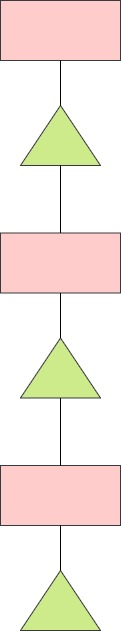
\includegraphics[width=2cm]{tree.jpg}
\]
		\item When translating a subclass hierarchy in an ER model into the relational model, the O-O approach always produces more relations than the direct-ER approach. Justify or prove otherwise. You may use the answer to part (a).\\
        \textbf{ANWSER}: ER Approach has exactly the same number of tables as the number of entity sets, which equals to n+1. However, the smallest number of relations one can get from O-O Approach is n+1. However, it is possible that the OO approach produces the same number of relations as direct-ER approach does. So the statement is partially correct.
	\end{enumerate}
\end{enumerate}


\section{ER Models}
Consider the following information about a music database.

\begin{enumerate}
\item There are many songs in the database, and each has a unique identification number 'SOIN', a name, a genre, and a release date. Each song is sung by one or more singers, is produced by exactly one production company, and can belong to one or more albums. In addition, some songs are purely instrumental, and in this case, they have one additional attribute, instrument.
\item Each song may end up winning zero or more awards. Each award is identified by the award name and year, and also has other attributes prize money and sponsor. The same award can be given to different songs.
\item Each production company has a unique company name, the date it was founded, and is run by exactly one president who is associated with a unique identification number 'PIN', name, gender, and age; each president can run multiple companies.
\item There are different departments in each production company, and they are uniquely identified by their department names, department numbers, as well as the company to which they belong.
\item Each singer is assigned a unique identification number 'SIN' and has a name, gender, language, and age as part of their information.
\item Each album has a unique identification number 'AIN', a name, and a year of publication. It can include one or more songs.
\end{enumerate}

Design and draw an ER diagram that captures the aforementioned information. Underline the primary key of each entity set. Try to be as succinct as possible-brevity will be rewarded. In particular, try to avoid adding additional unnecessary entity sets.

You are free to use annotation tools such as Mac Preview or Microsoft PowerPoint to draw the ER diagrams. Please do not include scanned hand-drawn pictures.\\
\\

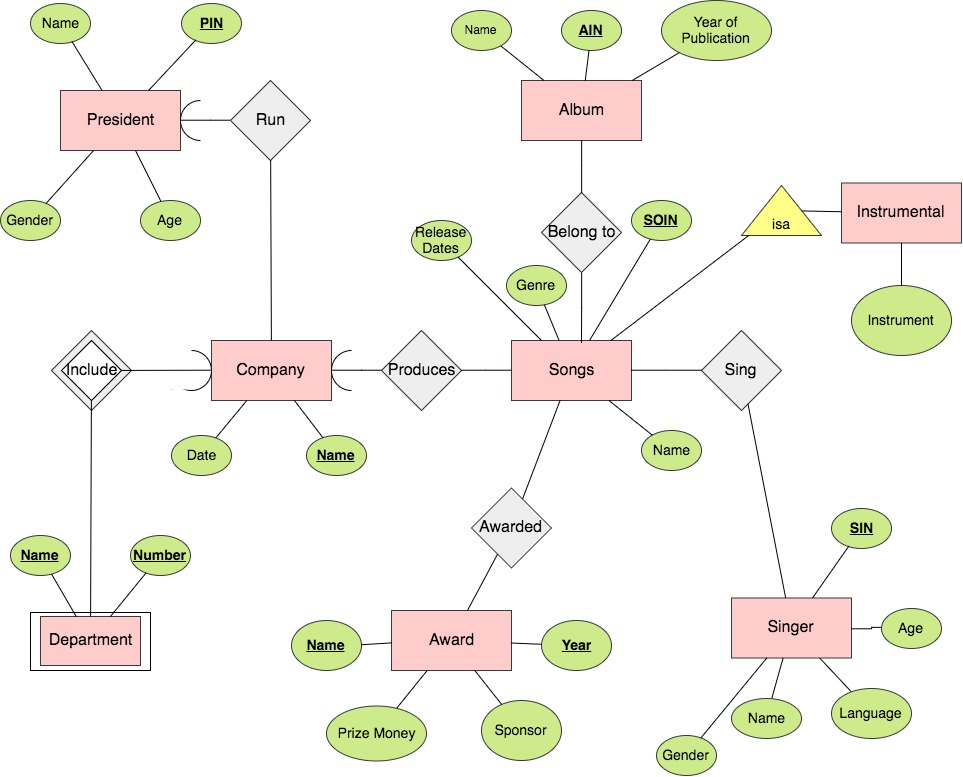
\includegraphics[width=\textwidth]{CS411HW1.jpg}\\
\\

\section{Relational Model}
Convert the ER model from the previous question to a relational model. For translating the subclass hierarchy, use the straight-ER approach. Please underscore the primary key of each entity, and merge relations as far as possible to minimize redundancy.\\

\noindent\fbox{%
    \parbox{\textwidth}{%
    	Songs(\underline{SOIN}, Name, Genre, ReleaseDates, Singer.SIN, Company.Name, Album.AIN)\\
        Instrumental(\underline{SOIN}, Instrument)\\
        Singers(\underline{SIN}, Age, Name, Gender, Language)\\
        Award(\underline{Name}, \underline{Year}, PrizeMoney, Sponsor)\\
        Company(\underline{Name}, date)\\
        President(\underline{PIN}, Name, Gender, Age)\\
        Album(\underline{AIN}, Name, YearofPublication)\\
        Department(\underline{Name}, \underline{Number}, \underline{Company.Name})
    }%
}

\section{DDL Commands}
Consider the following relational schema:
\begin{lstlisting}
Professor(NetID, name, department, officeAddress, officePhone, email) 
Student(NetID, name, department, graduationYear)
\end{lstlisting}
\begin{enumerate}
	\item Write the DDL commands that define each schema as a table in a relational database.\\
    \begin{lstlisting}
    	CREATE TABLE Professor(
    		NetID           VARCHAR(10) PRIMARY KEY,
        	name            VARCHAR(100),
        	department      VARCHAR(100),
        	officeAddress   VARCHAR(100),
    		officePhone     VARCHAR(20),
        	email           VARCHAR(20)
    	);
    \end{lstlisting}
    
    \begin{lstlisting}
    	CREATE TABLE Student(
    		NetID           VARCHAR(10) PRIMARY KEY,
        	name            VARCHAR(100),
        	department      VARCHAR(100),
    		graduationYear  INT(4)
    	);
    \end{lstlisting}
    
    \item Assuming these tables are created, write queries to (a) delete the graduationYear attribute from the Student table and (b) add an attribute GPA to the Student table, setting its default to 4.0.\\
    \begin{lstlisting}
    ALTER TABLE Professor DROP graduationYear;
    \end{lstlisting}
    
    \begin{lstlisting}
    ALTER TABLE Student ADD GPA FLOAT(4) DEFAULT 4.0;
    \end{lstlisting}
\end{enumerate}


%%% End document
\end{document}